% !TeX root = ../thesis.tex

%%%%%%%%%%%%%%%%%%%%%%%%%%%%%%%%%%%%%
\thesischapter[ch:introduction][0.8\textwidth]
  {``The more eyes, different eyes, we can use to observe one thing,\\ the more complete will our `concept' of this thing, our `objectivity,' be.''}
  {--- Friedrich Nietzsche, 1887, translated from German}
  {Introduction}
%``Je mehr Augen, verschiedne Augen wir uns für dieselbe Sache einzusetzen wissen, um so vollständiger wird unser 'Begriff' dieser Sache, unsre 'Objektivität' sein.''
\nocite{nietzsche1967genealogy}
\chapterabstract{This chapter introduces the scientific and statistical context of the thesis and motivates the need for principled microbiome data analysis. Microbiome data can be examined from several complementary perspectives, ranging from community-level summaries to feature-level measures and association networks. Rather than treating these perspectives as separate analysis tasks, the chapter organizes them into a coherent conceptual framework for comparative microbiome studies. It further introduces permutation testing as a recurring inferential tool across these analysis targets, before summarizing the main contributions of the thesis: the \texttt{NetCoMi} framework for microbial network analysis, the \texttt{permApprox} framework for improved permutation p-value approximation, and an integrated application to the PASTURE cohort.}
\chaptercontents

%%%%%%%%%%%%%%%%%%%%%%%%%%%%%%%%%%%%%

%====================================
\section{Microbiome data as statistical objects}
%====================================

Microbes are an integral part of our world. Long before humans began to systematically study them, they had already colonized almost every conceivable habitat on Earth. They live in soils and sediments, drive element cycles in oceans and freshwater systems, colonize plant surfaces and root systems, and persist in extreme environments such as deep-sea hydrothermal vents, polar ice, and acidic hot springs \citep{whitman1998prokaryotes, bar-on2018biomass, thompson2017communal,
fierer2017embracing, %soil microbiome
sunagawa2015structure, %ocean
trivedi2020plant, %plant
anesio2017microbiome}. %microbes in glaciers and polar ice
Their ecological reach even extends into the atmosphere, where vast and highly variable numbers of microorganisms occur as biological aerosols and can be transported over regional to intercontinental distances, linking distant habitats through continuous dispersal \citep{santl-temkiv2022microbial}.
In terms of abundance, prokaryotic microorganisms are estimated to number on the order of $10^{30}$ cells worldwide and constitute a substantial fraction of Earth’s total biomass, particularly in soils, oceans, and the deep subsurface \citep{whitman1998prokaryotes,bar-on2018biomass}. Together, these observations underscore that microbial communities are not marginal components of ecosystems but foundational drivers of planetary processes.

Within this broad ecological perspective, the human body represents another complex habitat for microbial life. Diverse microbial communities colonize specific parts of the body, including the gastrointestinal tract, oral cavity, skin, respiratory tract, and urogenital tract. These communities vary substantially across individuals and body sites, yet they are consistently present in healthy hosts \citep{turnbaugh2007human,hmp2009nihHMP}. The collective assemblage of microorganisms inhabiting a given environment is commonly referred to as the \emph{microbiota}, whereas the term \emph{microbiome} is often used in a broader ecological sense that encompasses not only the microorganisms themselves but also their collective genomes, functional capacities, metabolic activities, and interactions with their surrounding environment \citep{berg2020microbiome,xia2024applied}. 

Over the past two decades, the human microbiome has received increasing scientific and public attention due to its close relationship with host development and physiology. Microbial communities contribute to nutrient metabolism, immune system maturation, and colonization resistance against pathogens, and have been implicated in a wide range of diseases, including inflammatory, metabolic, and neurological disorders \citep{hooper2012interactions,gevers2014treatmentnaive,aggarwal2023microbiome,turnbaugh2006obesity}. Reflecting this functional integration, the human microbiome has been described metaphorically as an ``invisible organ'', highlighting its systemic relevance \citep{baquero2012microbiome,xia2024applied}.

The emergence of high-throughput sequencing technologies has fundamentally reshaped microbiome research. Following the transition from first-generation Sanger sequencing to massively parallel next-generation sequencing platforms, DNA sequencing became dramatically faster, more scalable, and substantially less expensive \citep{goodwin2016coming,shendure2017dna}. These advances enabled the direct sequencing of microbial genetic material without prior cultivation, overcoming a central limitation of classical microbiology. In particular, marker-gene amplicon sequencing and shotgun metagenomic sequencing allow researchers to characterize microbial communities on a large scale, providing complementary views on taxonomic composition and functional potential across diverse habitats \citep{sharpton2014introduction}.
Landmark efforts, including the Human Microbiome Project, have illustrated that systematic and reproducible profiling of microbial diversity across body sites and populations is not only possible but scalable to population-level studies \citep{hmp2009nihHMP,hmpconsortium2012structure}. As a consequence, microbiome research has evolved from small-scale descriptive studies into data-intensive investigations spanning thousands of samples and features. 

However, the ability to generate sequencing data on an increasingly large scale does not automatically translate into reliable scientific insight. Microbiome data exhibit structural characteristics that challenge many assumptions underlying classical statistical methodology. Sequencing experiments typically produce high-dimensional count matrices in which the number of microbial features may exceed the number of samples, a large proportion of taxa are rare, and zero counts are prevalent. In addition, because sequencing data provide information on relative rather than absolute abundances, the resulting observations are commonly treated as compositional: conditional on the sample-specific library size, the components are constrained to sum to a constant, inducing dependence between features even in the absence of biological interaction \citep{gloor2017microbiome}. These properties complicate modeling, inference, and interpretation in fundamental ways.

Consequently, even seemingly straightforward analyses require careful methodological consideration. Standard normalization strategies or classical hypothesis tests, if applied without accounting for sparsity, compositional constraints, and high dimensionality, may yield biased or misleading conclusions \citep{mcmurdie2014waste,weiss2017normalization}. The need for statistically principled approaches to microbiome data has therefore become widely recognized and has contributed to the emergence of \emph{microbiome statistics} as a distinct methodological field \citep{xia2024applied}. At the same time, the scientific questions driving microbiome research are typically comparative and hypothesis-oriented: researchers seek to understand how microbial communities differ across environments, interventions, or disease states, and which observed differences reflect robust biological signals rather than technical artifacts or random variation. Addressing such questions demands statistical frameworks that explicitly acknowledge the structural complexity of microbiome data and the different resolutions at which inference may be formulated.

The methodological developments presented in this thesis arise from precisely this intersection between biological complexity and statistical structure. Starting from the challenge of learning and comparing microbial networks under compositional and high-dimensional constraints, the work gradually exposes more fundamental inferential limitations related to resampling-based hypothesis testing. In this sense, the thesis traces a conceptual trajectory from network learning to improved permutation-based inference, addressing statistical bottlenecks that extend beyond any single application domain.

%====================================
\section{Analysis targets in microbiome studies}
\label{sec:intro:levels}
%====================================


Microbiome data can be analyzed with respect to different statistical targets that reflect distinct levels of aggregation. 
The same count table may give rise to questions about global properties of the microbial community, characteristics of individual taxa, or relationships between taxa. 
To provide a coherent conceptual organization, we distinguish three primary analysis targets: \emph{community-level summaries}, \emph{feature-level measures}, and \emph{association networks}. 
These targets represent increasing structural complexity, ranging from aggregated summaries to representations of the relationships between taxa. Orthogonal to the analysis target is the \emph{mode of analysis}. 
At each target, one may either characterize a single population or compare two or more groups. Single-population analysis aims to describe properties within a cohort, whereas comparative analysis assesses differences between groups defined by environmental, clinical, or experimental factors. In this thesis, we focus on the comparison between two groups.

Figure~\ref{fig:levels_inference} summarizes this organization. 
The columns represent the three analysis targets, while the rows distinguish between single-population and comparative analyses. A more detailed overview of the three targets is given below. The figure also highlights permutation testing as a cross-cutting tool for comparative analyses (Chapter~\ref{ch:permapprox}) and the integration of all components in a real-data application (Chapter~\ref{ch:application}). The numbers indicate the chapters in which the respective components are addressed.

\begin{figure}[!htb]
	\centering
	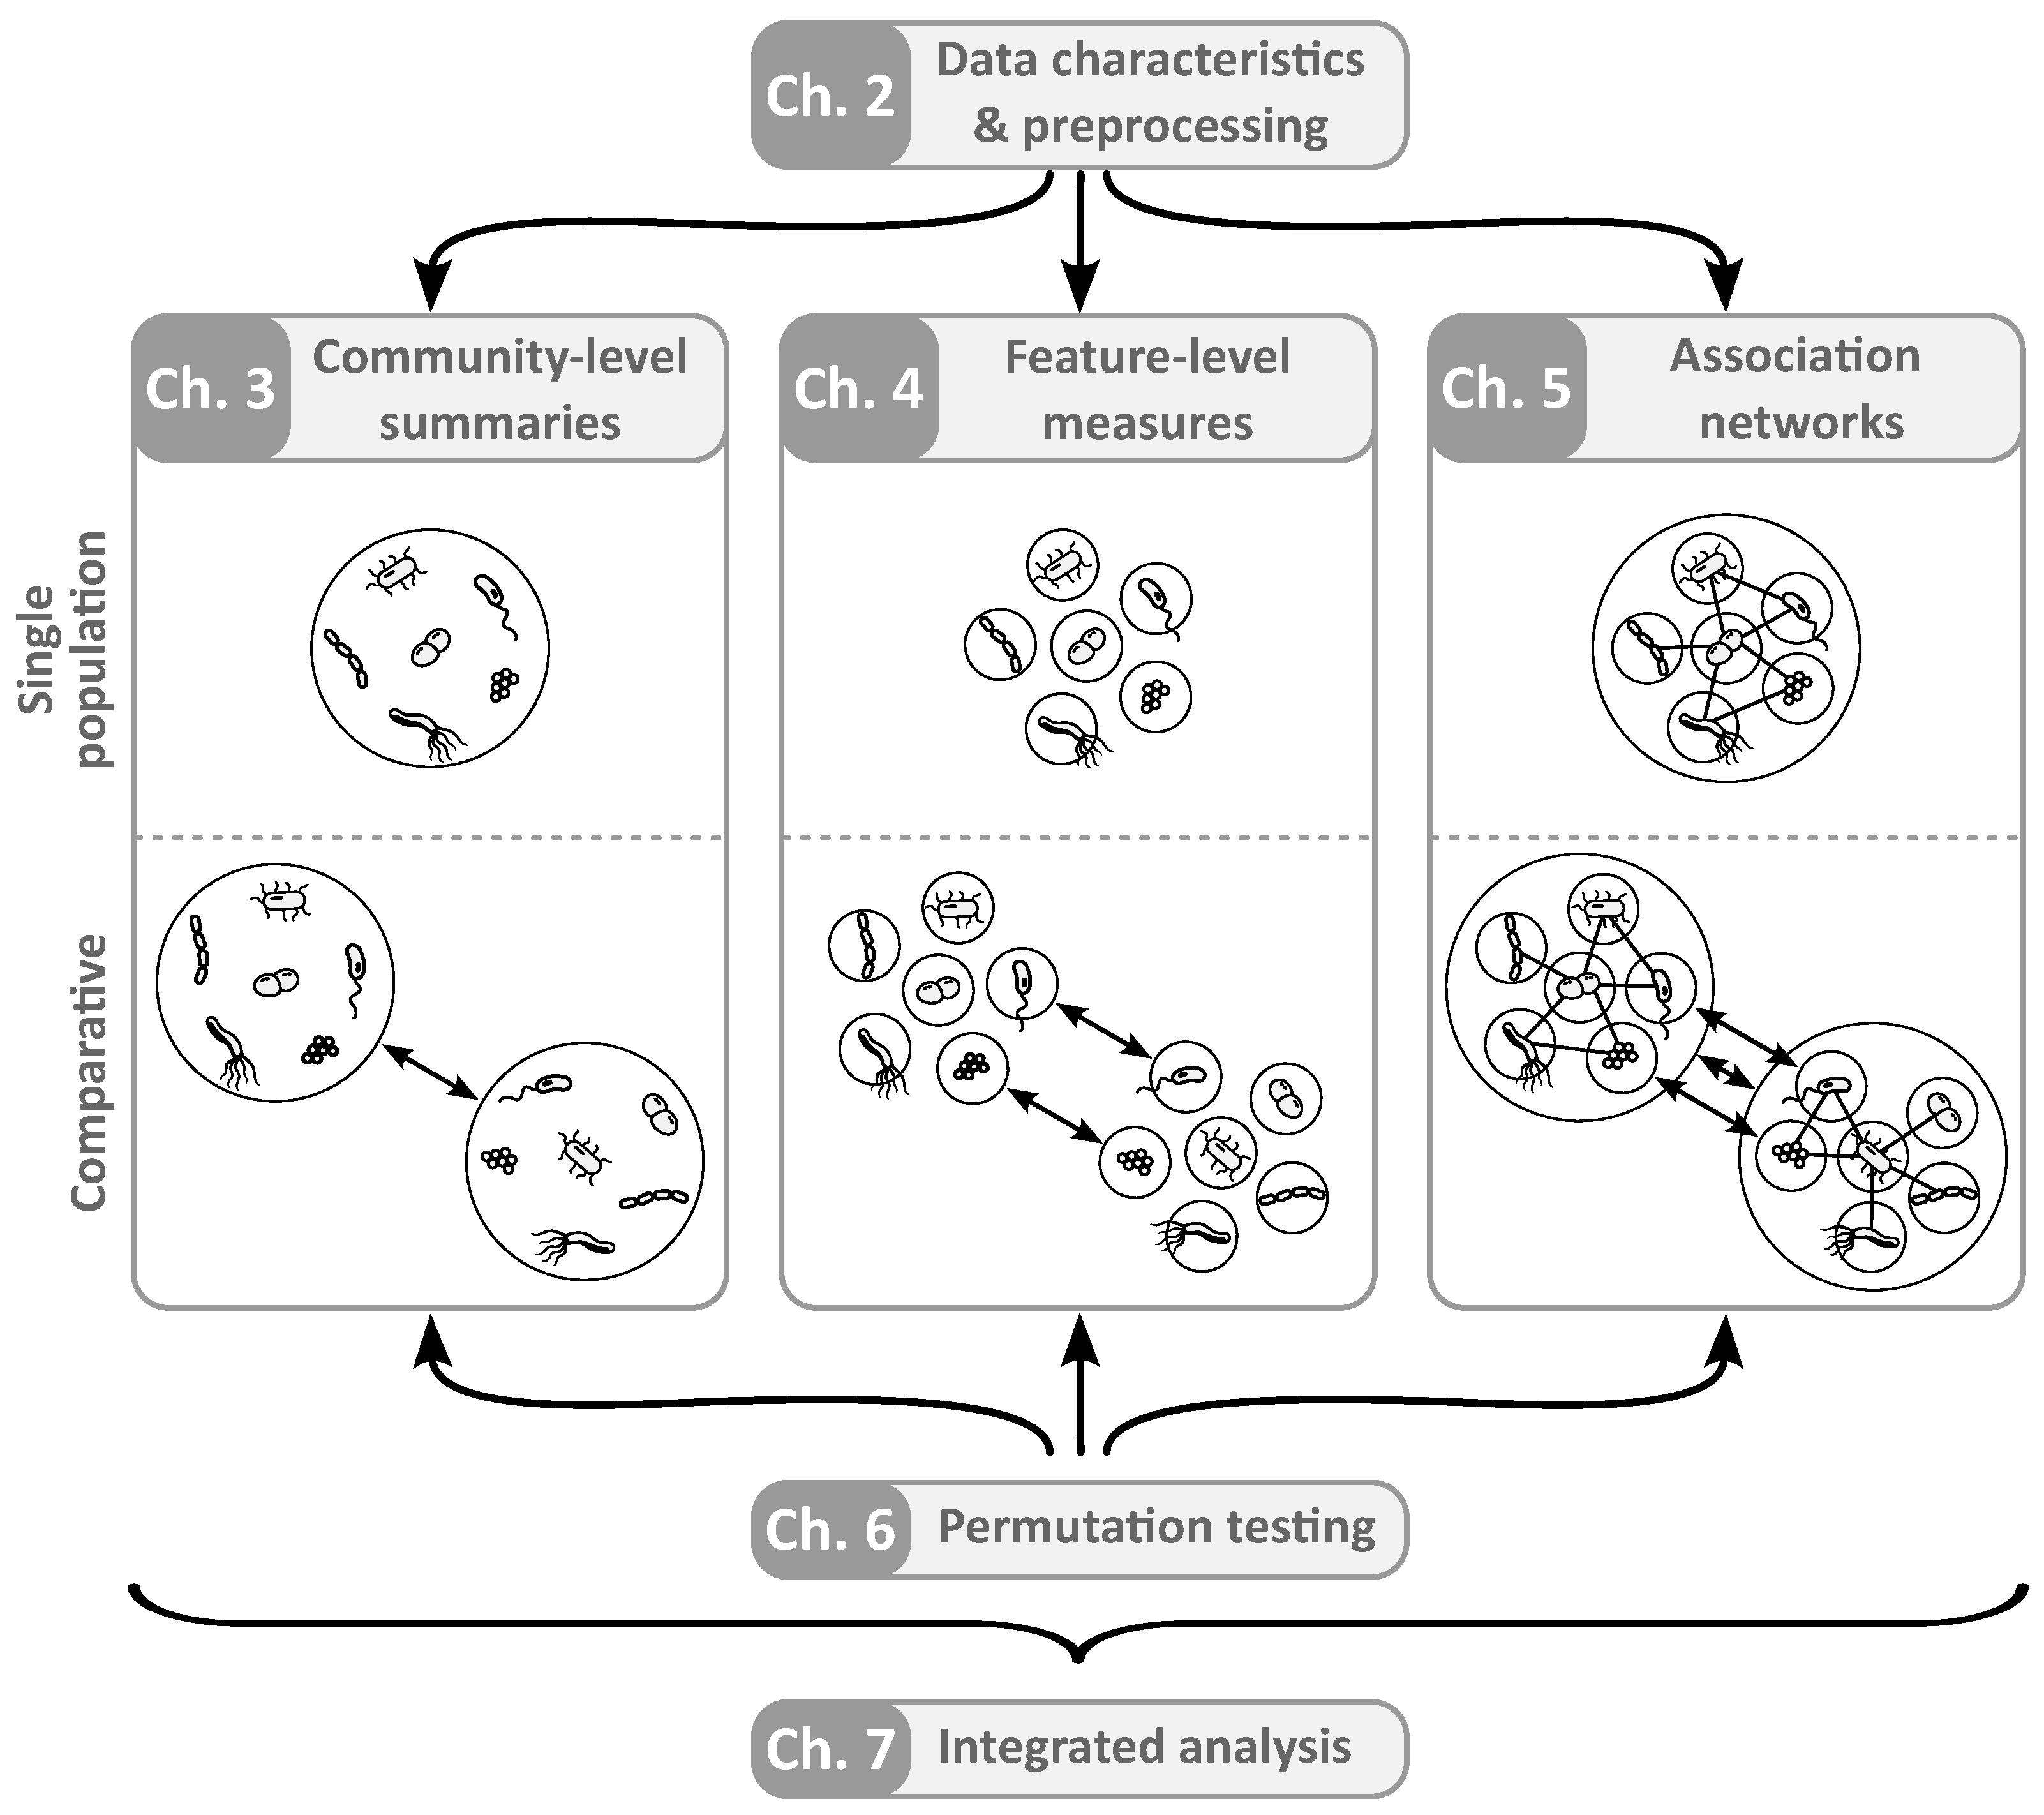
\includegraphics[width=\textwidth]{../ch01_introduction/figures/Intro_Figure.pdf}
	\caption{\textbf{Analysis targets and modes in microbiome studies.}
		The three columns represent the analysis targets considered in this thesis: community-level summaries, feature-level measures, and association networks. 
		The rows distinguish between single-population analysis and comparative analysis, where the latter focuses on differences between groups. 
		Data characteristics and preprocessing (Chapter~2) provide the foundation for all analysis targets. 
		Chapters~3 to 5 introduce methodological approaches for community-level summaries, feature-level measures, and association networks, respectively. 
		Permutation testing (Chapter~6) serves as a unifying inferential framework for comparative analyses across all targets. 
		Chapter~7 presents the complete analysis pipeline in an integrated real-data application.}
	\label{fig:levels_inference}
\end{figure}

\noindent\textbf{Community-level summaries.}
Community-level summaries describe aggregated properties of the microbial community. Typical quantities include measures of alpha diversity, such as richness or the Shannon index, as well as measures of beta diversity that quantify dissimilarity between samples. Ordination techniques provide low-dimensional representations of between-sample variation and facilitate exploratory analysis of community structure. In comparative settings, these summaries are used to assess whether global community characteristics differ between groups. 

\noindent\textbf{Feature-level measures.}
Feature-level measures characterize individual microbial taxa. 
In the single-population setting, this includes summaries of taxon abundances, prevalence patterns, and distributional characteristics within a cohort. In comparative settings, the objective is to quantify differences in abundance or distribution between groups or to assess associations with external covariates. Common approaches include differential abundance analysis, differential distribution testing, and regression-based modeling. All these methods operate at a marginal resolution, where each taxon is considered separately.

\noindent\textbf{Association networks.}
Association networks model relationships between microbial taxa. 
The primary object is a network whose edges encode statistical relationships, such as associations or conditional dependencies, between pairs of taxa. 
This relational representation gives rise to quantities at two complementary scales. 
On the one hand, node-level characteristics, such as centrality measures, describe the relative importance or role of individual taxa within the network. 
On the other hand, global network summaries, such as average path length or clustering coefficients, capture structural properties of the community as a whole. 
Association networks thus provide an explicitly relational perspective that links feature-level characteristics with community-level structure. 
As with the other analysis targets, network-based analyses can be performed within a single population or comparatively across groups, for example by assessing differences in network topology or in individual edges.


%====================================
\section{Permutation testing as a unifying approach}
\label{sec:intro:permutation}
%====================================

Across the different analysis targets introduced in the previous section, a common challenge arises in comparative settings: 
for many quantities of interest in microbiome analysis, the sampling distribution under the null hypothesis is analytically intractable or poorly approximated by classical parametric models. 
This difficulty is a direct consequence of the structural characteristics of microbiome data, including compositional constraints, sparsity, high dimensionality, and the use of complex transformations and derived statistics.

Permutation testing provides a general and flexible approach for hypothesis testing in such situations \citep{fisher1935design, good2005permutation}. Rather than relying on a parametric distribution, permutation tests approximate the null distribution by recomputing the test statistic under rearrangements of the data that preserve the null hypothesis. Their validity relies on exchangeability of the observations under the null hypothesis, which must be assessed with respect to the study design and the chosen permutation scheme \citep{good2005permutation}. Permutation tests are therefore useful in settings where classical distributional assumptions are difficult to justify.
Importantly, the relevance of permutation testing extends across all analysis targets considered in this thesis.

For community-level summaries, commonly used quantities such as alpha-diversity indices and between-sample dissimilarities often lack convenient parametric reference distributions. Group comparisons are therefore frequently based on nonparametric procedures. For example, PERMANOVA uses permutations of a distance-based test statistic to assess evidence for differences in multivariate community composition between groups \citep{anderson2001new}.

At the feature level, differential abundance and distribution analyses often involve sparse and discrete data, compositional transformations, or complex test statistics. In such settings, simple analytical reference distributions may be unavailable or may provide only an inadequate approximation to the null distribution.
Permutation-based approaches provide a robust alternative by directly approximating the null distribution of the chosen test statistic, regardless of its analytical form.

For association networks, permutation testing plays a central role in comparative analyses, as network characteristics typically lack tractable sampling distributions.
Permutation procedures are commonly used to assess differences in network structure, particularly for global network summaries and node-level characteristics whose sampling distributions are analytically intractable. Depending on the association measure and target of inference, edge-wise comparisons may alternatively be based on parametric or resampling-based procedures.

Taken together, permutation testing provides a unifying approach for hypothesis testing in comparative microbiome analyses across all considered targets. 
This central role motivates the methodological developments presented in Chapter~\ref{ch:permapprox}, where limitations of permutation-based testing under finite computational budgets are addressed and improved $p$-value approximation methods are developed.

%====================================
\section{Main contributions}
\label{sec:intro:contributions}
%====================================

At first glance, the methodological focus of this thesis may appear somewhat unexpected. 
Why concentrate on two seemingly distinct topics, namely microbial network analysis and permutation-based hypothesis testing? 
The former is a specialized tool within microbiome research, while the latter is a general statistical technique with applications far beyond this field. 
However, as will become apparent, both topics emerge naturally from the analytical challenges posed by microbiome data and are closely connected within comparative analysis workflows.

\subsubsection*{First contribution: a unified framework for microbial network analysis}
The focus on network analysis is perhaps the more intuitive of the two. 
Over the past decade, association networks have become a widely used exploratory tool for investigating relationships between microbial taxa and are increasingly incorporated into microbiome analysis workflows \citep{faust2021open}. 
At the same time, the literature reveals a lack of standardization, with microbial networks being constructed in many different ways and reflecting a wide range of methodological choices \citep{weiss2017normalization, kurtz2015sparse, ullmann2023overoptimism}. 
Their construction is inherently a multi-step procedure, involving preprocessing, association estimation, sparsification, and the computation of network characteristics. 
For each of these steps, a variety of methods exist.
Normalization strategies differ in their treatment of library size and compositional effects \citep{mcmurdie2014waste,mcknight2019methods,badri2020shrinkage}; compositionally aware association measures range from correlation-based methods to conditional-dependence approaches that can account for latent factors \citep{friedman2012inferring,quinn2017propr,kurtz2015sparse,kurtz2019disentangling}; and sparsification techniques include thresholding, shrinkage, and penalized likelihood procedures \citep{schafer2005shrinkage,meinshausen2006highdimensional,friedman2008sparse}. 

At the time of the original \texttt{NetCoMi} development, these methods were typically implemented in separate software packages and designed for specific components of the workflow rather than for integrated end-to-end analysis \citep{peschel2021netcomi}. Researchers therefore often had to assemble multiple methods in an ad hoc manner, limiting reproducibility and accessibility, especially for non-expert users.

To address these issues, the first methodological contribution of this thesis is the development of a unified framework for microbial network analysis. 
This framework is implemented in the \texttt{NetCoMi} \texttt{R} package \citep{peschel2026netcomi} and was introduced in \citet{peschel2021netcomi}. 
It provides an integrated workflow that guides the user from count data to a fully constructed and analyzed network by combining preprocessing, association estimation, sparsification, and network characterization within a single framework, while allowing flexible choices among established methods at each step. 
In addition, the framework supports comparative analyses, enabling the construction and comparison of networks across groups within a common and reproducible analytical framework. 
The \texttt{NetCoMi} framework is accompanied by comprehensive documentation and tutorials and has been integrated into the \emph{Orchestrating Microbiome Analysis} (OMA) workflow \citep{borman2024orchestrating}, where network-based methods are embedded into a broader microbiome analysis pipeline. 
By integrating existing methodology into a coherent and user-friendly framework, \texttt{NetCoMi} improves reproducibility, transparency, and accessibility of network-based microbiome analysis.

\subsubsection*{Second contribution: improved $p$-value approximation in permutation testing}
The second focus of this thesis, permutation-based hypothesis testing, arises less directly but is closely tied to comparative network analysis. 
When comparing microbial networks across groups, differences in network characteristics are typically assessed using permutation tests, as the underlying test statistics do not admit tractable parametric distributions. 
However, in this setting, two fundamental challenges emerge.

First, microbiome data are often high-dimensional, and network construction itself is computationally demanding. 
As a consequence, only a limited number of permutations can be performed in practice. 
This leads to empirical $p$-values that lie on a coarse discrete grid, resulting in limited resolution in the tail of the distribution \citep{north2002note, phipson2010permutation}. 
After multiplicity adjustment, this limited resolution can prevent small effects from being distinguished and may render adjusted significance thresholds unattainable unless a substantially larger number of permutations is used \citep{phipson2010permutation, gilbert2005modified}..

Second, while approaches based on extreme value theory, in particular generalized Pareto distribution (GPD) approximations, have been proposed to address this limitation \citep{knijnenburg2009fewer, winkler2016faster}, their practical application raises additional challenges. 
In preliminary investigations, existing GPD-based methods could still produce zero $p$-values when a negative estimated shape parameter implied bounded fitted support and the observed test statistic lay at or beyond the resulting upper endpoint.
Moreover, GPD-based approximation involves several methodological choices, including threshold selection and parameter estimation, for which a wide range of approaches has been proposed in extreme-value analysis \citep{scarrott2012review, langousis2016threshold, bader2018automated}, while guidance tailored specifically to permutation-based p-value approximation remains limited.

The second methodological contribution of this thesis addresses these challenges by developing a robust framework for permutation $p$-value approximation. 
This methodology is introduced in \citet{peschel2026permapprox} and implemented in the \texttt{permApprox} \texttt{R} package \citep{peschel2025permapprox}. 
The proposed approach ensures strictly positive $p$-value estimates by incorporating a support constraint into the GPD fitting procedure, thereby avoiding zero $p$-values. 
In addition, it provides a principled workflow for threshold selection and parameter estimation. 
Its performance is systematically evaluated through extensive simulation studies, showing accurate and stable $p$-value approximation across the simulated settings considered under limited permutation budgets.

Although the motivation for this development originates from comparative network analysis, the resulting methodology is formulated in a general way. 
It is applicable to permutation testing problems beyond network analysis and is relevant whenever $p$-values must be estimated from a limited number of permutations. 
This generality is reflected in the applications presented in this thesis, where the approach is used not only for network comparisons but also for analyses at the community and feature levels.

\subsubsection*{Third contribution: integrated real-data analysis across analysis targets}
The third contribution of this thesis is an integrated real-data analysis based on infant gut microbiome data from the PASTURE cohort \citep{vonmutius2006pasture}. It combines community-level summaries, feature-level comparisons, and association-network analyses within a coherent workflow. The analysis illustrates how complementary perspectives can yield distinct, but jointly informative, insights: taxa exhibiting marginal abundance differences are not necessarily central within association networks, and differential associations may occur without pronounced marginal group differences. By applying permutation-based procedures across the analysis pipeline and refining the resulting $p$-values with \texttt{permApprox}, the application also demonstrates the practical connection between the two methodological contributions of this thesis.

\subsubsection*{Reproducibility}
The code, analysis material, and figures accompanying this thesis are available in a GitHub repository archived on Zenodo \citep{Peschel2026thesisRepo}. The repository is structured by thesis chapter. Each chapter is represented by a corresponding folder containing the material used to generate or reproduce the reported results, tables, and figures. For chapters without accompanying analysis scripts, the corresponding folder contains the graphical material shown in the thesis. Large intermediate files from simulation studies are not included in all cases, but can be regenerated by rerunning the corresponding scripts provided in the repository.

Together, these contributions provide both methodological and practical advances for comparative microbiome research, linking workflow integration, permutation-based hypothesis testing, and applied analysis within a unified framework.

%====================================
\section{Thesis outline}
\label{sec:intro:structure}
%====================================

This dissertation follows a monograph structure that combines methodological development with applied microbiome data analysis.

\textbf{Chapter 2} formalizes microbiome sequencing data as statistical objects. It characterizes key properties of high-throughput sequencing data, including compositionality, sparsity, and high dimensionality, thereby establishing the foundations for the subsequent chapters.

\textbf{Chapter 3} introduces methods for community-level summaries. It presents commonly used measures such as alpha and beta diversity, along with ordination techniques, and discusses their use in descriptive and comparative analyses of microbial communities.

\textbf{Chapter 4} focuses on feature-level measures. It reviews approaches for analyzing individual taxa, including differential abundance and distributional analyses, and discusses statistical challenges arising from compositionality and sparsity.

\textbf{Chapter 5} focuses on association networks and presents the first methodological contribution of this thesis: the \texttt{NetCoMi} framework. 
It reviews existing approaches and introduces a unified workflow that integrates network construction, characterization, and comparison. 
Practical challenges arising from the implementation and combination of different methods are discussed throughout the chapter.

\textbf{Chapter 6} presents the second methodological contribution, a framework for accurate permutation $p$-value approximation under limited permutation budgets. It introduces the constrained tail-modeling approach, develops the associated workflow, and evaluates its performance in extensive simulation studies.

\textbf{Chapter 7} demonstrates the integration of the different analysis targets in a real-data application. Using a cohort study, it combines community-level summaries, feature-level measures, and association networks within a coherent analysis pipeline.

\textbf{Chapter 8} concludes the thesis with a discussion of the methodological contributions, their practical implications, and directions for future research.


Notation and abbreviations used throughout the thesis are summarized in Appendix~\ref{app:notation}. Chapter-specific notation is introduced locally where needed. In particular, Chapter~\ref{ch:permapprox} contains a dedicated overview for permutation testing and GPD tail modeling.
